\documentclass{article}
\usepackage[utf8]{inputenc}
\usepackage{fancyhdr}
\usepackage{graphicx}
\usepackage{hyperref}
\usepackage{geometry}


% ---- Commands ------- %
\newcommand{\documentNumber}[1]{
    \LARGE  \textbf{ PUSP2142{#1} } \\
    \medskip
}
\newcommand{\documentVersion}[1]{
    v.{#1} \\
    \medskip
}
\newcommand{\documentTitle}[1]{
    \centerline{\rule{13cm}{0.4pt}}
    \bigskip \bigskip
    \LARGE {#1} \\
    \bigskip \bigskip
    \centerline{\rule{13cm}{0.4pt}}
}
\newcommand{\documentGroup}[1]{
    \bigskip \bigskip
    \LARGE Group {#1} \\
    \bigskip
}
\newcommand{\documentResponsible}[1]{
    \LARGE Responsible: {#1} \\
    \medskip
}
\newcommand{\documentAuthors}[1]{
    \LARGE Authors: {#1} \\
    \medskip    
}
\newcommand{\documentDate}[1]{
    \date {#1} 
}


% --- Header & Footer ---- %
\pagestyle{fancy}
\lhead{\leftmark}
\rhead{}
\rfoot{\thepage}
\cfoot{}
\lfoot{}


% ------------------------------------------------ #


\title {
    \documentNumber {01}    % Must be 2 digits
    \documentVersion {0.1}
    \documentTitle {Software development plan - SDP}
    \documentGroup {2}
    \documentResponsible {(PG) Project Management Group}
    \documentAuthors {(PG) Project Management Group}
    \documentDate {2021-01-29}
}

\begin{document}

\maketitle
\thispagestyle{empty}

\newpage

\tableofcontents

\newpage

\section{Introduction}
    This document describes the development model and the development plan for !!NAME!!, 
    which will be a system for time reporting and is based on \textit{Baseblock System}.
    !!NAME!! will be developed by students at LTH in the course 
    \textit{ETSF20 Programvaruutveckling för stora projekt}.

\section{Terminology}
    \renewcommand{\arraystretch}{1.7}  % Vertical padding for tables
    
    \begin{table}[h]
        \centering
        \begin{tabular}{| p{1.5cm} | p{9cm} |}
            \hline
                Baseblock system & This is the base system that is used in !!NAME!! \\
            \hline
                SG & System architecture Group \\
            \hline
                DG & Developer Group \\
            \hline
                QG & Quality control Group \\
            \hline
                PG & Project management Group \\
            \hline 
                CML & Configuration Management List, consists of all configuration units \\
            \hline            
                ECG & Error Control Group, consists of PG and SG \\
            \hline
                SDP & Software Development Plan \\
            \hline
                SDP & Software Development Plan \\
            \hline
                SRS & Software Requirements Specification \\
            \hline
                SVVS & Software Verification and Validation Specification \\
            \hline
                SVVI & Software Verification and Validation Instruction \\
            \hline
                STLDD & Software Top Level Design Document \\
            \hline
                SDDD & Software Detailed Design Document \\
            \hline
                SVVR & Software Verification and Validation Report \\
            \hline
                SSD & System Specification Document \\
            \hline
        \end{tabular}
    \end{table}

\section{Referenced Documents}
    \begin{itemize}
        \item \href{https://google.github.io/styleguide/javaguide.html}{Google Java Style Guide}
        \item CML
    \end{itemize}
    

\section{Development Model} %Assar och Victor
    The development model that is used in this project is the waterfall model. This
    means that the project is divided into four seperate phases where each phase depends
    on the previous one in a sequential manner. It is thus required that a phase is
    completed before the next one begins.
    \\ \\
    In every phase, there are several documents that must be produced and a phase
    is considered completed only once all documents required in the phase has reached baseline.
    To reach baseline, all documents of the phase must first pass an informal review, 
    followed by a formal review.
    
\section{Staff Organisation} %Assar
    \subsection{Project Managment Group}
        \begin{itemize}
            \item Coordinating the group effort.
            \item Making a project schedule.
            \item Ensuring that every individual has the information they need.
            \item Authoring the following documents.
                \begin{itemize}
                    \item SDP
                    \item SSD
                    \item PFR
                \end{itemize} 
        \end{itemize}
    
    \subsection{Software Architecture Group}
        \begin{itemize}
            \item Designing the software architecture
            \item Delegating work to DG and QG.
            \item Coordinating and co-authoring of the following documents.
                \begin{itemize}
                    \item SRS
                    \item STLDD
                    \item SDDD
                    \item PFR
                \end{itemize}
        \end{itemize}
 
    \subsection{Development Group}
        \begin{itemize}
            \item Design GUI for the software.
            \item Develop the architecture that SAG designed.
            \item Co-author the following documents.
                \begin{itemize}
                    \item SRS
                    \item STLDD
                    \item STDDD
                    \item PFR
                \end{itemize}
        \end{itemize}
    
    \subsection{Quality Control Group}
        \begin{itemize}
            \item Testing and validating the functionality of code written by DG.
            \item Authoring the following docuemnts.
            \begin{itemize}
                \item SVVS
                \item SVVI
            \end{itemize}
            \item Co-authoring the following documents
                \begin{itemize}
                    \item SRS
                    \item PFR
                \end{itemize}
        \end{itemize}
        
    \subsection{Others}
        The forementioned groups make up the team resposible for developing the software. Other stakeholders include. 
        \begin{description}
            \item [Head of section] Overseas the project and has direct contact with the client. 
            \item [Client] Provides a requirement specification.
            \item [Experts] Provides auxiliary knowledge in their respective fields. 
            \item [Examiner] Performs the formal review.
        \end{description}
\newpage

\section{Schedule}
    The project starts at week 3 and ends in week 12, which means that
    there are 9 weeks available to work. Figure \ref{schedule} illustrates
    the estimated time for each phase and the estimated days for meetings,
    informal reviews and formal reviews.
    
    \begin{figure}[h]
        \centering
        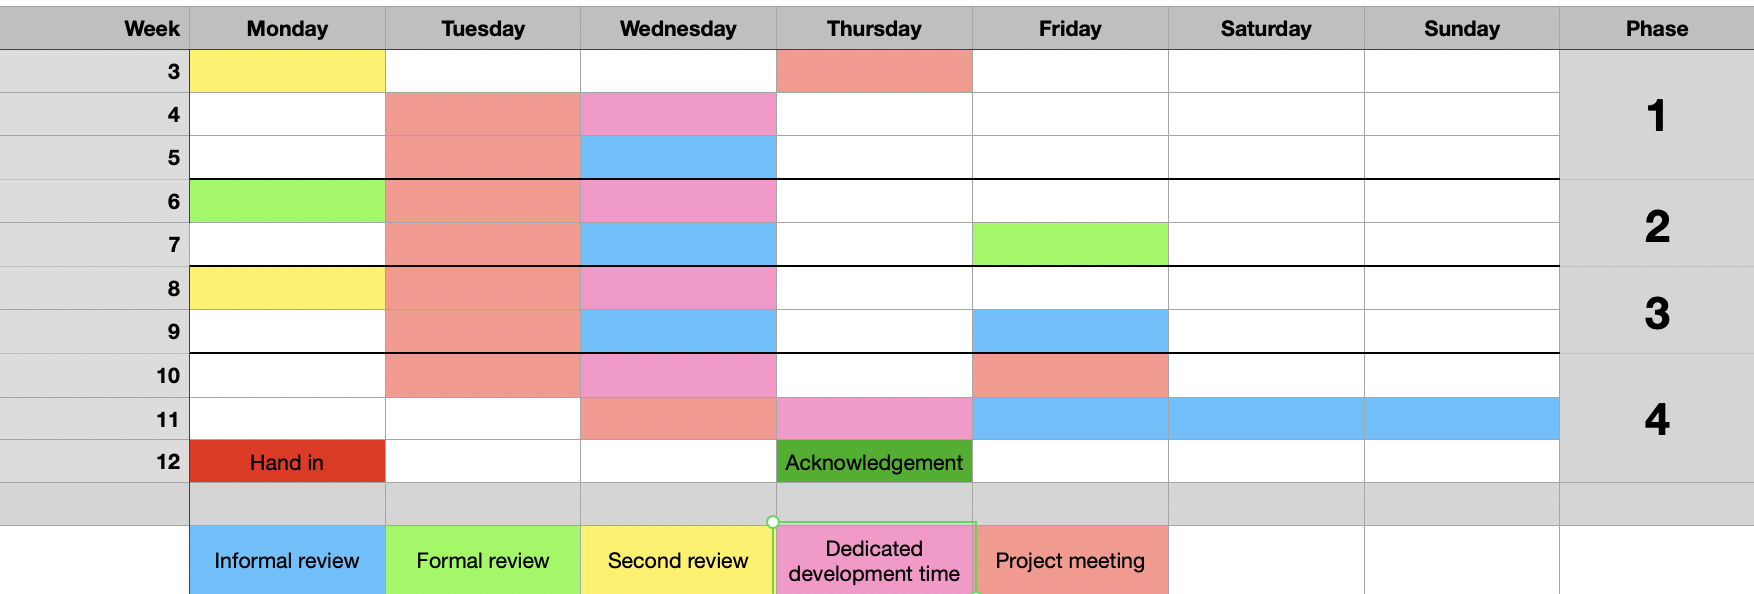
\includegraphics[width=\textwidth]{images/schedule.png}
        \caption{Estimated project schedule}
        \label{schedule}
    \end{figure}
    
    On Tuesdays there are Project group Meeting \label{PM}, which mandatory for every member in the group.
    On these meetings the project is discussed and general decisions can be taken. This is an important
    step in the development model, to ensure that everyone is on the same page and that the time plan
    is being kept.
    
    
    \subsection{Estimated Work Load}
        PG holds one hour long meeting every week and has scheduled for a two hour time slot every wednesday where every group works on their respective task. To supplement this, the groups are expected to hold their own planing meetings and work sessions. Since the workload of each group varies between phases, it seemed more fitting to allow groups the flexibility of managing their own time. Group leaders have been tasked with making sure that coordination between groups is constant throughout the project. PG also estimated that approximately an hour every week will be spent on general discussions in the discord channel.
        \\ \\
        Table \ref{phasetable} illustrates the estimated start and end dates 
        for every phase, as well as estimated hours spent per week, per person.
        \begin{table}[h]
            \centering
            \begin{tabular}{|c|c|c|c|c|}
                \hline
                    \textbf{Phase} & \textbf{Start} & \textbf{End} & \textbf{Work days} & 
                    \textbf{Estimated hours/week} \\
                \hline
                    1 & 18/1 & 5/2 & 15 & 10 \\
                 \hline
                    2 & 08/2 & 19/2 & 10 & 10 \\
                 \hline
                    3 & 22/2 & 5/3  & 10 & 10 \\
                 \hline
                    4 & 8/3 & 19/3  & 10 & 15 \\
                 \hline
            \end{tabular}
            \caption{Estimated start and end for the phases}
            \label{phasetable}
        \end{table}
        \\
        Table \ref{activitytable} illustrates the estimated time spent per
        activity as well as how often the activity is expected to occur.
        
        \begin{table}[h]
            \centering
            \begin{tabular}{|l|c|c|}
                \hline
                    \textbf{Activity} & \textbf{Frequency/week} & \textbf{Duration (h)} \\
                \hline
                    Project group meeting & 1 & 1 \\
                 \hline
                    Project group work & 1 & 2 \\
                 \hline
                    Subgroup work session & 2 & 2*2 \\
                 \hline
                    Self studies & 1  & 1 \\
                 \hline
                    Discussions & 1 & 1 \\
                 \hline
                    Reviews/Expert meetings & 1 & 1 \\
                 \hline
                    \textbf{Total hours} & & \textbf{10} \\
                 \hline
            \end{tabular}
            \caption{Estimated time for each activity per person, per week}
            \label{activitytable}
        \end{table}
    

\section{Standards \& Tools}    % Victor
    In order to make the development process as easy and straight forward as possible,
    the project group has agreed on several standards and tools to use. 
    \\ \\
    The standards should be followed by every group member and consists of the following:
    \begin{itemize}
        \item The soure code should follow the
        \href{https://google.github.io/styleguide/javaguide.html}{Google Java Style Guide}.
        \item All comments, commits and pull-requests should be in english.
    \end{itemize}
    
    \subsection{Discord}
    Discord is used as the many communcation tool in the group. A server has been setup and is
    used for both messaging, working together and having project meetings.
    The server consistst of several voice channels and several text channels, each
    with its specific purpose, eg "Meetings" or "Developer Group".
    
    \subsection{Github \& Git}
    Git is used for collaboration between decouments and the project library (see \ref{project_library})
    and is hosted on Github. Git provides abilities that  makes certain action very
    easy, such as pulling and pushing updates to the working repository and creating pull-requests for merging.
    
    \subsection{Eclipse}
        Eclipse is the primary IDE that is used due to its familarity in
        the group and its huge span of different properties such as plugins.
    
        \subsubsection{Egit}
            Egit is a plugin for Eclipse that provides the tools needed for a git workflow 
            in Eclipse IDE.
            
        \subsubsection{Texmaker}
            Texmaker is a latex edtiro that provides the tools needed to compile and preview latex files.
    
\section{Follow up and Quality Evaluation}
    To keep the quality of all documents as high as possible during the project,
    two reviews will be carried out and the end of every phase. One informal review
    followed by one formal review.

    \subsection{Informal Review \label{informalreview}}
        The informal review is performed within the project group and is meant to catch
        errors, bugs or mistakes in the documents. This is to ensure as high quality
        as possible for the formal review. The result of the review is \emph{not} pass or
        not pass, but its purpose is rather to improve the documents.
        \\ \\
        The informal review is carried out 3 days before the formal review and the documents that
        shall be reviewed should ready at latest 17:00 the day before the review. PG is responsible
        for coordinating the meetings as well as documenting it.
        There are at least three reviewers assigned for each document to be reviewed, and these
        are assigned by PG. During the review the reviewers will mention and discuss what they have
        found and then the reviewees will ge an opportunity to reply and have a potential discussion
        if needed.
        \\ \\
        To emphasize, the informal review is \emph{not} ment to criticize or judge, but rather
        to make the documents as good as possible.
        
    
    \subsection{Formal Review \label{formalreview}}
        Once the documents have passed the informal review, they must pass the formal review
        to reach baseline. During the formal review, and extern reviewer is
        given the documents at least 48 hours in advance so that he or she can prepare.
        During the actual review, the entire project group shall be present.
        The formal review can result in one of the four scenarios:
        \begin{enumerate}
            \item The documents are approved
            \item The documents are approved after certain modification.
            \item Modifications must be made followed by a re-review.
            \item The documents are \emph{not} approved and must be re-written,
                    followed by a new review.
        \end{enumerate}
    
    \subsection{Re-Review}
        In case the documents fail the formal review, it might be necessary to
        to do a new review after certain modifications have been made.
            
    \subsection{Following the Timeplan}
        
            Det  ska  finnas  en  del  i  projektplanen  som  beskriver  hur  uppf ̈oljning,  t  ex  avtidplanen,  sker under projektet,  samt vad som h ̈ander om arbetet inte verkarg ̊a enligt plan.  

\section{Configuration Managment}   % Victor
    All changes to units in the CML must follow a certain procedure once the documents
    are in baseline. Git and Github are the main tools that are used to handle configuration management in this project.

    \subsection{Project Library \label{project_library}}
        The project library consists of two seperate libraries: Document libray and Work library.
    
        \subsubsection{Document Library \label{doclibrary}}
            The document library consists of the following:
            
            \begin{itemize}
                \item All configuration units that have reached baseline.
                \item All documents that invloves version control and change management (see                       section \ref{versioncontrol}).
                \item Protocols from informal reviews (see section \ref{informalreview}).
                \item Protocols from formal reviews (see section \ref{formalreview}).
                \item Protocols and agendas from Project Group Meetings (see section \ref{PM}).
            \end{itemize}
            \noindent
            The purpose of this library is that the customer or a reviewer at any point should be able to access these documents. 
            This means that this library is initially almost empty, and documents are added as the project proceeds. In the end of phase 4, all units found in CML can be found in this library.

            
        \subsubsection{Work Library}
            The work library contains everything all files that are required during the project.
            The library is divided into three different branches where each branch has a unique purpose.
            
            \begin{itemize}
                \item \begin{verbatim} development \end{verbatim}
                This branch is where the all development is done and is used as a placement for all files related
                to the project, regardless of the documents status.
                Every member in the group has free push access to this branch.
                
                \item \begin{verbatim} review \end{verbatim}
                Once the documents in the development branch are ready for a formal review,  they are moved
                into the \textit{review} branch. This requires a pull-request to be made, which must be reviewed and accepted by ECG before it is merged into the branch. 
                
                \item \begin{verbatim} master \end{verbatim}
                Once the documents pass the formal reviews, they are merged into 
                \textit{master} branch, which consists of only files that have reached baseline.
                Once new documents are added to this branch, they are also placed in the document library (see section \ref{doclibrary}).
                Note that not all files are copied to the document library, but only the documents specified in the CML.
                
            \end{itemize}
            
            \begin{figure}[h]
                \centering
                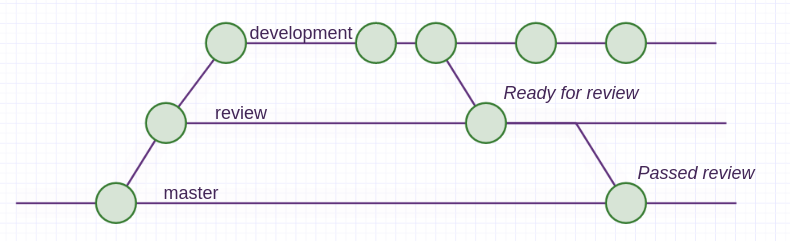
\includegraphics[width=\textwidth]{images/workflow.png}
                \caption{Workflow of the three branches.}
                \label{workflow}
            \end{figure}
        
    \subsection{Version Control \label{versioncontrol}}
        Once a configuration unit has reached baseline there are several steps
        that must be taken in order to make changes to it.
        These steps consists of the following:
        \begin{enumerate}
            \item Creating a error report that states what the
                    error is with the unit, in its current state.
            \item The error report is handed to the ECG who creates a 
                    status report. ECG then decides if the error is legitimate.
            \item If the error is deemed legitimate, then they
                    propose a solution and
                    decides whom shall be responsible to fix the problem.
                    Once the error is corrected, ECG must approve it
                    and then the unit version must be updated.
                    The status report is then closed.
            \item If ECG decides that the error is to be discarded, then
                    the problem and status report is closed.
                
        \end{enumerate}

    \subsection{Version naming \& update}
        
        
    


\section{Rules and Guidelines} %Assar
    To ensure clear communcation and efficiency PG has set up a series of rules and guidelines. 
    
    \begin{description}
        \item[React to information] Discord has a feature that allows users to react to messages with an emoji. This is a good way to let the sender know that their message has been acknowledged.
        \item[Mandatory attendance for group meetings and work sessions] If a group member is unable to attend a meeting they are expected to contact PG and get the information another way.  
        \item[Weekly time report in epuss every Friday 17:00]
        \item[All project documents are written in English]
        \item[ ]
    \end{description}
    

        

Det ska finnas en del i projektplanen som beskriver hur uppföljning, t ex av
tidplanen, sker under projektet, samt vad som händer om arbetet inte verkar
gå enligt plan. Det ska också finnas en beskrivning av de rutiner som finns för
kvalitetsutvärdering under projektet.

    

\section{Risk Analysis}

    Table \ref{risktable} illustrates some of the possible risks that the projects
    faces as well as their likelhood of happening and their possible impact.
    \\
    The scale is \textbf{Low} $\rightarrow$ \textbf{Mid} $\rightarrow$ \textbf{High}.





    I projektplanen ska även resultatet av en riskanalys för projektet presenteras.
    Ange hur riskanalys utförts i projektet, samt de viktigaste riskerna som identi-
    fierats. rapportera åtminstone följande för varje rapporteras risk: skattad san-
    nolikhet (t ex, låg, medel, hög), skattad effekt (t ex, låg, medel, hög), möjliga
    indikatorer på att risken förvekligas, samt exempel på lösningar om risken för-
    verkligas.
    \begin{table}[h]
        \centering
        \begin{tabular}{|l|l|l|l|}
            \hline
                Risk & Probability & Impact & Solution \\
            \hline
            Lack of communication & High & High 
                & \parbox{.45\textwidth}
                {\begin{itemize}
                    \item Be very clear \emph{where} we communicate
                    \item Everyone will pay extra attention to all communication channels
                        in use.
                    \item Ensure that the other part of the communcation has recieved
                        and understood the information.
                    \item Active listening, ask for confirmation.
                    \item Ask questions.
                 \end{itemize}}\\
            \hline
            Poor work distribution & High & Medium 
                & \parbox{.45\textwidth}
                {\begin{itemize}
                    \item Everybody takes resposibility for their work.
                    \item Communicate with your group leader.
                    \item Even distribution of work.
                    \item If you finish early, ask if anybody needs help. 
                    \item Ask for help if you are falling behind.
                 \end{itemize}}\\
            \hline
            Poor planning & High & Medium 
                & \parbox{.45\textwidth}
                {\begin{itemize}
                    \item Plan around deadlines
                    \item Consider individual schedules
                 \end{itemize}}\\
            \hline
            Probelms with the document library & Medium & Medium 
                & \parbox{.45\textwidth}
                {\begin{itemize}
                    \item Hold lectures breaking down the steps
                    \item Use cheat sheats and provide additional resources
                 \end{itemize}}\\
            \hline
            Personal conflicts within the group & Medium & Medium 
                & \parbox{.45\textwidth}
                {\begin{itemize}
                    \item Put your pride aside and focus on a solution.
                    \item Have understanding for others.
                    \item Tell a leader if you feel like you are being treated unfairly.
                    \item Ask somebody to mediate in a conflict
                 \end{itemize}}\\
            \hline
        \end{tabular}
        \caption{A break down of risks and measures taken to avoid them}
    \end{table}
    
\end{document}
